Es wird  in  Detail  beschrieben,  welche  elektronische Komponenten aus welchem
Grund ausgew\"ahlt worden sind.

% **************************************************************************** %
\subsection{36V Netzteil und Netzeingang}
% **************************************************************************** %

Die  maximale Ausgangsleistung wurde grob berechnet  mit  $\SI{24}{\volt}  \cdot
\SI{3}{\ampere} = \SI{72}{\watt}$.

Da das Aufbauen eines eigenen Netzteils zu aufw\"andig und teuer gewesen w\"are,
entschieden wir uns f\"ur  ein  externes  Netzger\"at dass im Geh\"ause montiert
werden kann. Das verwendete Netzteil  liefert  \SI{36}{\volt} und \SI{75}{\watt}
und ist in der Abbildung  \ref{fig:circuit:mains-input}  als \emph{N2} zu sehen.

\begin{figure}[th!]
    \center
    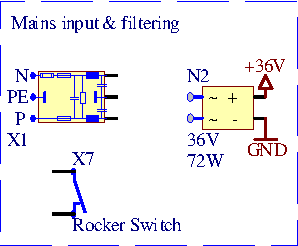
\includegraphics[width=.35\textwidth]{images/circuit/mains-input.pdf}
    \caption{Netzspannung wird gefiltert und auf 36V DC durch ein externes Netzmodul transformiert}
    \label{fig:circuit:mains-input}
\end{figure}

Weiter  wird eine Netzeingangs-Steckverbinder mit  integriertem  Netzfilter  und
Sicherung  verwendet,  was  in  der Abbildung \ref{fig:circuit:mains-input}  als
\emph{X1}  zu  sehen ist. Ein  auf  der  R\"uckseit  des  Geh\"auses  montierter
Schalter  \emph{X7}  erlaubt  das  Ein-  und   Ausschalten   des   Endproduktes.

% **************************************************************************** %
\subsection{Spannungsversorgungen}
% **************************************************************************** %

F\"ur die digitale  Logik  werden  die  zwei  Spannungspegel  \SI{5}{\volt}  und
\SI{3.3}{\volt} ben\"otigt. 

\begin{figure}[th!]
    \center
    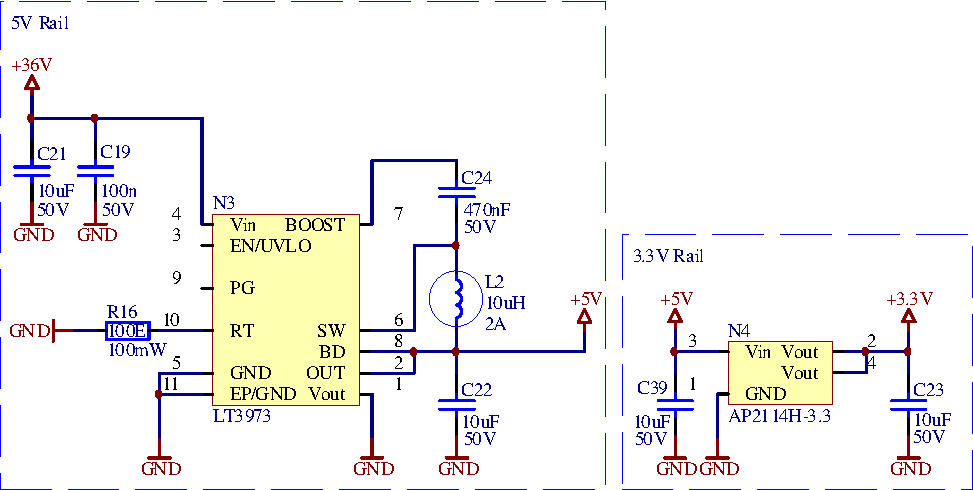
\includegraphics[width=.75\textwidth]{images/circuit/5v-3v-rails.pdf}
    \caption{Speisung f\"ur 5V mittels Abwertswandler (links) und Speisung f\"ur 3.3V mittels Linearregler (rechts)}
    \label{fig:circuit:rails}
\end{figure}

Die  \SI{36}{\volt} vom Netzteil werden mittels eines getakteten  DC-DC-Wandlers
auf \SI{5}{\volt} transformiert,  was  in  der Abbildung \ref{fig:circuit:rails}
vom Bautil \emph{N3} verwirklicht wird.

Die \SI{3.3}{\volt} werden im Gegensatz von einem Linearregler \emph{N4} erzeugt
damit die  \SI{3.3}{\volt}  Speisung  m\"oglichst  St\"orfrei  ist. Somit sollte
verhindert  werden, dass die DACs und ADCs verrauscht sind bzw. ungenau  messen.

% **************************************************************************** %
\subsection{LT3741}
% **************************************************************************** %

Der  Spannungswandler  f\"ur  die  Ausgangsspannung  ist  das Herzst\"uck dieser
Schaltung.

Die  Ausgangsspannung   muss   mindestens   im  Bereich  von  \SI{0}{\volt}  bis
\SI{24}{\volt}  liegen  und   einen  Rippel  kleiner  als  \SI{300}{\milli\volt}
besitzen.  Der  Ausgangsstrom muss mindestens im Bereich von \SI{0}{\ampere} bis
\SI{3.5}{\ampere} liegen  und  einen  Rippel kleiner als \SI{100}{\milli\ampere}
besitzen. Dabei  sollte  die Effizienz bei Volllast mindestens \SI{80}{\percent}
betragen.

Da  das  Endprodukt  schlussendlich  in  Serie  mit  mehreren   Spannungs-  oder
Stromquellen  geschalten  werden  k\"onnte, muss  zus\"atzlich  darauf  geachtet
werden,  dass  der Spannungswandler \emph{leistungsaufnahmef\"ahig}  sein  muss.
Diese Eigenschaft weist  ein  sogenannter  \emph{Synchronwandler}  vor und wurde
zusammen mit den Spannungs-,  Strom-,  und Leistungsanforderungen als prim\"ares
Merkmal f\"ur die Produktsuche eines Wandlers verwendet.

Der   \emph{LT3741}    erf\"ullt    alle   Anforderungen.   In   der   Abbildung
\ref{fig:circuit:buck} ist der Aufbau zu sehen.

\begin{figure}[th!]
    \center
    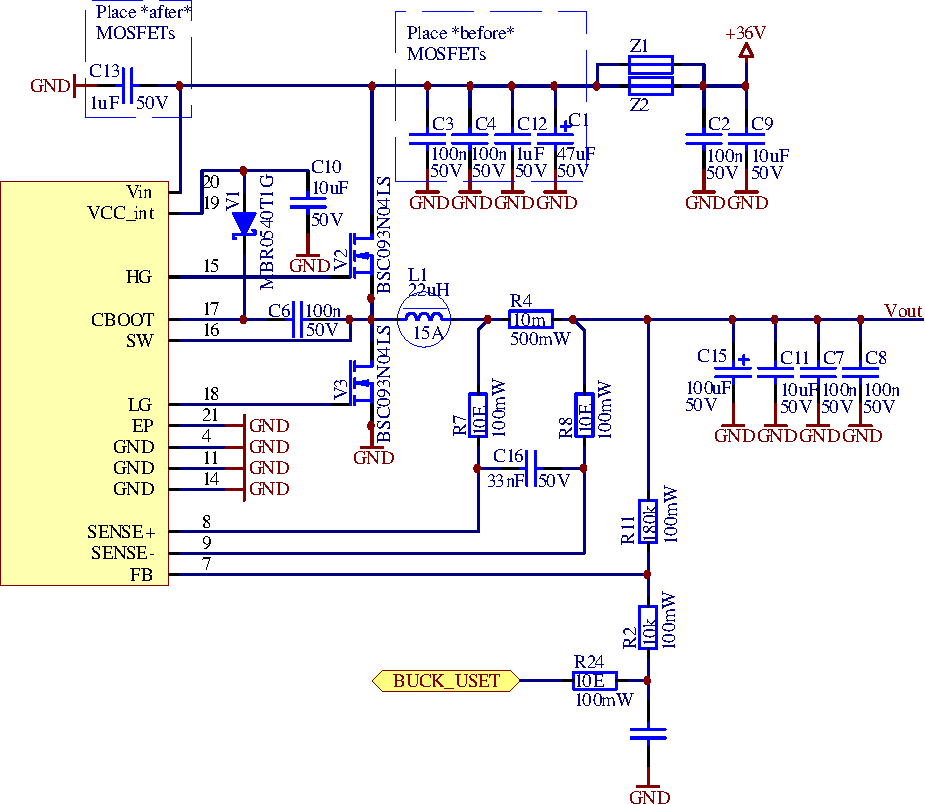
\includegraphics[width=.75\textwidth]{images/circuit/buck.pdf}
    \caption{Herzst\"uck des Projektes: Aufbau des LT3741 CVCC Synchronwandler}
    \label{fig:circuit:buck}
\end{figure}

Der  \emph{LT3741}  wird  mit  \SI{36}{\volt}  gespiesen  (oben  rechts  in  der
Abbildung \ref{fig:circuit:buck}). Da diese Schaltung  viel  St\"orung  auf  der
\SI{36}{\volt}     Speisung    verursachen    w\"urde,    werden    verschiedene
Keramikkondensatoren  und Ferritkerne verwendet, um  die  hochfrequente  Signale
m\"oglichst zu eliminieren und somit die  anderen  Speisungen davon zu bewahren.

Die Bauteile \emph{V1}  und  \emph{C6}  bilden zusammen mit dem MOSFET \emph{V2}
ein High-Side-Switch.

\begin{figure}[H]
    \center
    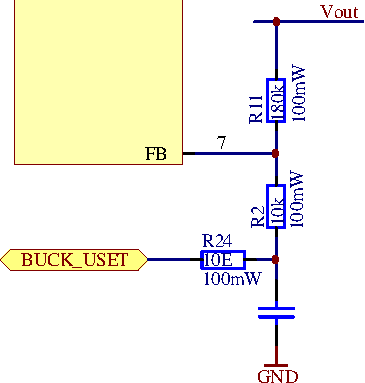
\includegraphics[width=.35\textwidth]{images/circuit/buck-uset.pdf}
    \caption{Einstellung der Ausgangsspannung durch \"Anderung der Bezugsspannung im Feedback-Loop mittels einer analogen Steuerspannung von 0V bis 1.5V}
    \label{fig:circuit:buck:uset}
\end{figure}

\begin{figure}[H]
    \center
    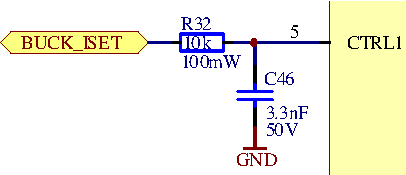
\includegraphics[width=.4\textwidth]{images/circuit/buck-iset.pdf}
    \caption{Einstellung des Maximalstroms mittels einer analogen Steuerspannung von 0V bis 1.5V}
    \label{fig:circuit:buck:iset}
\end{figure}

\begin{figure}[H]
    \center
    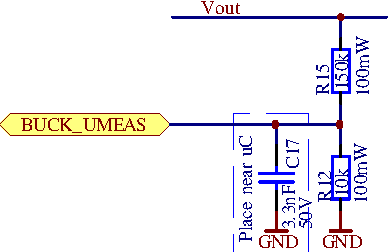
\includegraphics[width=.45\textwidth]{images/circuit/buck-umeas.pdf}
    \caption{Messen der Ausgangsspannung}
    \label{fig:circuit:buck:umeas}
\end{figure}

\begin{figure}[H]
    \center
    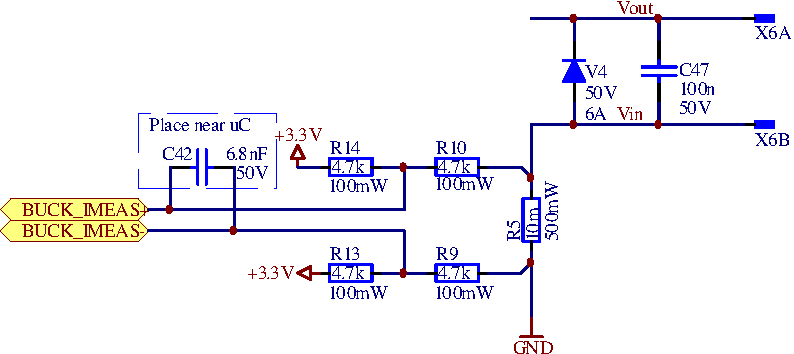
\includegraphics[width=.85\textwidth]{images/circuit/buck-imeas.pdf}
    \caption{Messen des Ausgangsstromes}
    \label{fig:circuit:buck:imeas}
\end{figure}

\begin{figure}[H]
    \center
    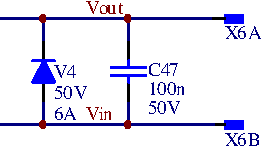
\includegraphics[width=.35\textwidth]{images/circuit/output-connectors.pdf}
    \caption{Verpolungsschutz am Ausgang}
    \label{fig:circuit:output}
\end{figure}

\begin{figure}[H]
    \center
    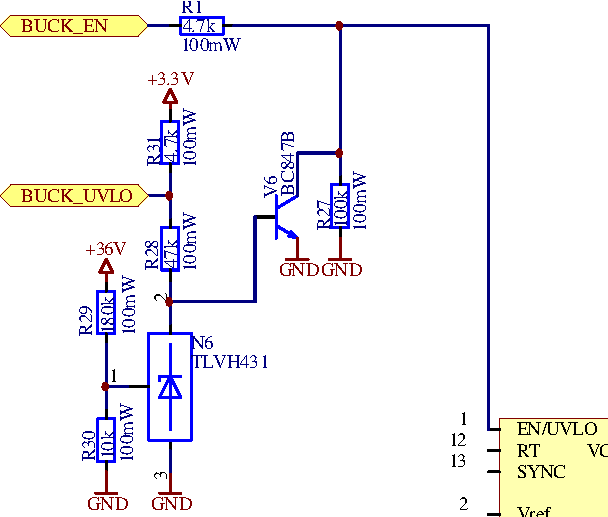
\includegraphics[width=.6\textwidth]{images/circuit/uvlo.pdf}
    \caption{Under-Voltage Lock-Out (UVLO) erm\"oglicht ein kontrolliertes Ein- und Ausschalten des Reglers}
    \label{fig:circuit:uvlo}
\end{figure}

\begin{figure}[H]
    \center
    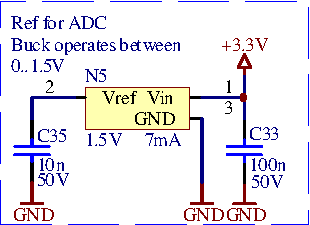
\includegraphics[width=.4\textwidth]{images/circuit/vref.pdf}
    \caption{1.5V Referenzspannung um die ADCs m\"oglichst in Full-Range betreiben zu k\"onnen}
    \label{fig:circuit:vref}
\end{figure}

\begin{figure}[H]
    \center
    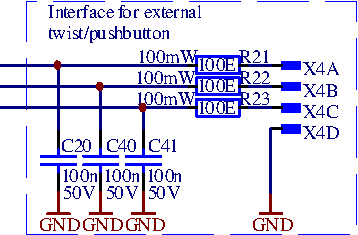
\includegraphics[width=.4\textwidth]{images/circuit/pushbutton.pdf}
    \caption{Drehdruckknopf}
    \label{fig:circuit:pushbutton}
\end{figure}

